\section{Type Hole Inference}
\label{sec:thi}

While local type inference reduces the number of necessary annotations, 
constraint-based type inference as found in languages like ML and Haskell allows programmers to omit most or all type annotations \cite{HM, pierce}. The trade-off is that type error localization and recovery 
become considerably more difficult, because inconsistencies can now arise between 
constraints derived from many distant locations in a program. 
Heuristic approaches, e.g. based on manually tuned weights or machine learning methods, are necessary to intelligently guess which uses of a variable are what is  intended.\todo{cites}

This is reminiscent of the situation considered in Sec.~\ref{sec:conditionals}\todo{cite} of inconsistent branches in a conditional, but there is no parent expression where we can localize the inconsistency. However,
this gives us a hint at the approach we introduce in this section: we \emph{gradually} harmonize local and constraint-based type inference. In particular, our \emph{type hole inference} approach generates constraints after the bidirectional process as described in the previous sections finishes. We then unify, recovering from inconsistent constraints by localizing the problem 
to \emph{type holes} that cannot be solved by constraint unification and computing a graph of partial solutions. The user can interactively investigate various partial solutions to clarify their intent, which might allow local type inference to localize the error to the relevant expressions. \todo{subsec refs}

% We define "solving" the constraints associated with a given type hole as the process of (1) identifying all of its possible type fillings and (2) reporting the most informative fillings to the user. If all possible fillings are consistent with each other and do not elicit occurs check failure, the type hole is deemed \emph{solvable}.

\subsection{Type Hole Inference in Hazel}
% Taking advantage of the interactive nature of live programming, rather than inferring sources of blame, we simply ask the user. \emph{Type hole inference} displays all possible sources of inconsistency and allows the user to identify which to blame. Once a user attempts to fix the program, the editor can display new errors as they arise. In this manner, the program can be iteratively and interactively repaired.

In Figure \ref{fig:editor_holes}, the user has written an incomplete program where the function $f$ is annotated with a type hole. Using type hole inference, the editor displays the inferred type for $f$ in gray. The return type is not constrained, so it is left unknown here (see below on polymorphic generalization).
\begin{figure}[H]
\includegraphics[width=9cm]{images/example_holes.png}
\includegraphics[width=9cm]{images/example_holes_CI.png}
\caption{Incomplete program with partial hole filling suggestion}
\label{fig:editor_holes}
\end{figure}
Figure \ref{fig:editor_conflict} demonstrates visual feedback shown when a type hole is \textit{unsolvable}. The type hole is highlighted in red and marked with a bang (\li{!}). The user is informed via the Type Inspector that the type hole cannot be solved due to conflicting information from constraints. Figure \ref{fig:editor_conflict} shows how the editor could temporarily fill the type hole when the user hovers over a constraint, deferring to bidirectional error localization from there. (This interaction has not yet been implemented, but there is no barrier to doing so. For our experiments, copy/paste was used to simulate.)
\begin{figure}[H]
\includegraphics[width=9cm]{images/example_conflict.png}
\includegraphics[width=9cm]{images/example_conflict_CI.png}
\includegraphics[width=9cm]{images/example_conflict_hover.png}
\includegraphics[width=9cm]{images/example_conflict_hover_CI.png}
\caption{User types '2' and error is localized to type hole. Error is localized to '2' when hovering over a selection, which transiently fills the hole [interaction mocked up for presentation]}
\label{fig:editor_conflict}
\end{figure}
% \begin{figure}[H]
%   \includegraphics[width=9cm]{images/example_conflict_hover.png}
% \includegraphics[width=9cm]{images/example_conflict_hover_CI.png}
% \caption{user hovers over conflicting constraint to show origin [mock-up]}
% \label{fig:editor_conflict_hover}
% \end{figure}
Figure \ref{fig:editor_ghost} illustrates a program which has a full solution for $f$'s type annotation. The user can then press the Tab key to accept the suggested filling for the type hole.
\begin{figure}[H]
\includegraphics[width=9cm]{images/example_ghost.png}
\includegraphics[width=9cm]{images/example_complete_CI.png}
\includegraphics[width=9cm]{images/example_complete.png}
\caption{User removes '2' and types 'true' in the else branch before accepting the new suggestion}
\label{fig:editor_ghost}
\end{figure}
% \begin{figure}[H]
% \includegraphics[width=9cm]{images/example_complete.png}
% % \includegraphics[width=9cm]{images/example_complete_CI.png}
% \caption{user accepts hole filling suggestion}
% \label{fig:editor_complete}
% \end{figure}

\subsection{Unique Identifiers for Holes}

\label{sec:typinf}
We must be able to uniquely identify type holes when constraint solving because we will treat type holes as type inference variables. Thus, we make two small changes to the marked lambda calculus's syntax:
\[\begin{array}{rrcl}
    \Prov & \Provp & \Coloneqq & u \mid exp(u) \mid \rightarrow_L(\Provp) \mid \rightarrow_R(\Provp)\\
    \TMName  & \TMV  & \Coloneqq & \dots \mid \TUnknown^{p}\\
    \ECMName & \ECMV & \Coloneqq & \dots \mid \ECUnboundId{x}{u} \mid \ECInconTypeId{\ECMV}{u} \mid \ECInconBrId{\ECMV}{\ECMV}{\ECMV}{u} \mid \EEHole^u
\end{array}\]

\begin{enumerate}
    \item We add a unique id $u$ to all expression holes and type holes that appear directly in the program. We assume that id generation is handled by the editor.
    \item Type holes can also arise internally during constraint generation, below. To identify these, we generalize unique IDs to \emph{provenances}, $p$. These serve two useful but non-critical purposes:
\begin{enumerate}
    \item Provenances establish how each type hole connects to some type hole or expression hole that lies in the program. For instance, the provenance $exp(3)$ tells us that this type hole is the synthesized type of the expression hole with id 3. We discuss the matched arrow provenances below. Future user interface affordances could use provenances to better identify holes, e.g. when internal holes appear in the type or context inspector.
    \item Provenances allow increased efficiency when compared to generating fresh type hole ids (which spawns larger constraint graphs during constraint generation.) 
\end{enumerate}
\end{enumerate}
% These changes are depicted in Figure ~\ref{fig:adjusted-calculus-syntax}.
% \begin{figure}[htbp]
%   % \[\begin{array}{rrcl}
%   %   \Prov & \Provp & \Coloneqq & u \mid exp(u) \\
%   %   \TMName  & \TMV  & \Coloneqq & \TUnknown^{p} \mid \TNum \mid \TBool \mid \TArrow{\TMV}{\TMV} \\
%   %   \ECMName & \ECMV & \Coloneqq & x \mid \ECLam{x}{\TMV}{\ECMV} \mid \ECAp{\ECMV}{\ECMV}
%   %                      \mid           \ECNumMV \mid \ECPlus{\ECMV}{\ECMV}
%   %                      \mid           \ECTrue \mid \ECFalse \mid \ECIf{\ECMV}{\ECMV}{\ECMV} \\
%   %            &       & \mid         & \ECUnbound{x}^u \mid \ECInconType{\ECMV}^u \mid \ECInconBr{\ECMV}{\ECMV}{\ECMV}^u \mid \EEHole^u
%   % \end{array}\]
  
%   \caption{Adjusted syntax of the marked lambda calculus}
%   \label{fig:adjusted-calculus-syntax}
% \end{figure}

\subsection{Constraint Generation}
The first step is constraint generation. Our approach closely follows the usual approach \cite{TAPL0}, by augmenting the bidirectional type system for the marked lambda calculus with generated constraint sets, $C$. The new judgement forms are 
    $\synConstraint{\ctx}{\ECMV}{\TMV}{C}$ and $\anaConstraint{\ctx}{\ECMV}{\TMV}{C}$. 

\subsubsection{Constraints}
Individual constraints are written $\tau_1 \approx \tau_2$. 
The relationship that a constraint expresses is not quite consistency, nor is it equality. Rather, if $\tau_1 \approx \tau_2$, $\tau_1$ and $\tau_2$ must have the same solution once the constituent type holes are filled. The constraint relation is reflexive and symmetric. It also behaves transitively, but only through type holes and types containing type holes. We refer to such types as "incomplete" types, following \citet{HazelnutPOPL}.

% Before detailing this relationship, consider an approach where constraints were transitive across complete types. In such a world, we may end up with the incorrect error localization below:
% \begin{center}
% \includegraphics[width=4cm]{images/constraint_gen_bad_example.png}
% \end{center}
% This program can be associated with the constraints $C = \{ \tehole^{x} \approx \tnum, \tehole^{y} \approx \tnum, \tehole^{y} \approx \mathtt{string} \}$ based on the usage of the $+$ operator and binding of $"hello"$ to $y$. Since the editor treats constraints as transitive across complete types, it finds that $\tehole^{x} \approx \tehole^{y}$ given $\tehole^{x} \approx \tnum$ and $\tehole^{y} \approx \tnum$. Consequently, the two type holes have conflicting type hole fillings of $\tnum$ and $\mathtt{string}$. This behavior is undersirable, as $\tehole^x$ was not directly associated with the string $"hello"$ and should be solved as $\tnum$.

As an example of the constraint generation process, let us consider the program illustrated in Figure \ref{fig:editor_ghost}. We define an equivalent marked expression $\ECMV_{ex}$ below where the let expression has been replaced with an annotated lambda applied to the let body:
$$\ECMV_{ex} = \ECAp{(\ECLam{f}{\TUnknown^1}{~~\ECIf{\EEHole^2~}{~(\ECAp{f}{\underline{2}})}{~\EEHole^3}})}{~~\EEHole^0}$$
What constraints might we expect this expression to generate? In this expression, we expect that the annotation of the lambda is consistent with the type of its argument, $\TUnknown^{exp(0)}$. This notion might generate the constraint $\{ \TUnknown^1 \approx \TUnknown^{exp(0)}\}$. We might further notice that we expect both branches of the if expressions to synthesize consistent types. But what is the type of $\ECAp{f}{\underline{2}}$? Previously, we might have argued that it would simply be $\TUnknown$; however, now we must ask exactly \emph{which} type hole this application synthesizes and determine its provenance. In order to further understand these questions, let us more formally explore constraint generation before revisiting this example.

\subsubsection{Subsumption Constraints}
% As discussed earlier, constraints constitute a series of expectations for what different types should be. One key mechanism by which we facilitate our accumulation of these expectations is analysis. Indeed, when we expect something should have a type \TMV, we commonly analyze it against that type. As a classic example of this, consider subsumption. 

Suppose we have a marked expression \ECMV~ that satisfies the judgement \ctxSynType{\ctx}{\ECMV}{\TMV'} for some context \ctx. If we attempt to analyze \ECMV~ against the type $\tau$, we require, or put another way, we expect, that \consistent{\TMV}{\TMV'}. We extend the rule MASubsume as follows so that it generates the corresponding constraint $\tau \approx \tau'$:
\begin{mathpar}
  \judgment{
    \synConstraint{\ctx}{\ECMV}{\TMV'}{C} \\
    \consistent{\TMV}{\TMV'} \\
    \subsumable{\ECMV}
  }{
    \anaConstraint{\ctx}{\ECMV}{\TMV}{C \cup \{ \TMV \approx \TMV'\}}
  }{MASubsume-C}
\end{mathpar}
% Notice that we also accumulate constraints generated in each premise in our conclusion.

One key question is how one should manage constraints whenever marked expressions are marked with errors. Should an expected type pass through the mark, which would necessarily create an unsolvable constraint? We assert that the answer is no: marks  act as quarantines. We can, however, take advantage of the interpretation of marks as non-empty holes to infer a type for the marked expression, i.e. the type that mark repair needs to target.

With this guiding principle in hand, let us approach constraint generation for subsumption when \inconsistent{\TMV}{\TMV'} by extending MAInconsistentTypes:
\begin{mathpar}
  \judgment{
    \synConstraint{\ctx}{\ECMV}{\TMV'}{C}  \\
    \inconsistent{\TMV}{\TMV'} \\
    \subsumable{\ECMV}
  }{
    \anaConstraint{\ctx}{\ECInconTypeId{\ECMV}{u}}{\TMV}{C \cup \{ \TMV \approx \TUnknown^{exp(u)} \}}
  }{MAInconsistentTypes-C}
\end{mathpar}
% Here, instead of expecting that the type of \ECMV~ be consistent with the type $\tau$, we prevent any conflicts that may arise from $\tau$ reaching beyond our type hole membrane. We then enforce that the hole surrounding \ECMV~ synthesize a type consistent with $\tau$.

\subsubsection{If Expressions and Their Constraints}
Expectations for the result of typechecking on expressions is not limited to analysis. Indeed, there are multiple cases where we hold expectations for the types of our expressions in synthesis as well. As a simple example, consider if expressions. We expect that both branches have consistent types and assess this implicitly by attempting to compute their join. This leads to the following constraint generating rule for if expression synthesis where we simply accumulate constraints and require that $\TMV_1 \approx \TMV_2$:
\begin{mathpar}
  \judgment{
    \anaConstraint{\ctx}{\ECMV_1}{\TBool}{C_1}  \\
    \synConstraint{\ctx}{\ECMV_2}{\TMV_1}{C_2} \\
    \synConstraint{\ctx}{\ECMV_3}{\TMV_2}{C_3}
  }{
    \synConstraint{\ctx}{\ECIf{\ECMV_1}{\ECMV_2}{\ECMV_3}}{\TJoin{\TMV_1}{\TMV_2}}{C_1 \cup C_2 \cup C_3 \cup \{ \TMV_1 \approx \TMV_2 \}}
  }{MSIf-C}
\end{mathpar} 

Our logic is somewhat trickier when the branches of an if expression have no lower bound, causing it to be wrapped in a marked hole. Inconsistency among branches should be considered an error that lies \emph{within} the hole membrane surrounding our marked expression. Consequently, we constrain $\TMV_1 \approx \TMV_2$ as before and do not consider the type of our hole membrane, $\TUnknown^{exp(u)}$, in the constraints:
\begin{mathpar}
  \judgment{
    \anaConstraint{\ctx}{\ECMV_1}{\TBool}{C_1} \\
    \synConstraint{\ctx}{\ECMV_2}{\TMV_1}{C_2} \\
    \synConstraint{\ctx}{\ECMV_3}{\TMV_2}{C_3} \\
    \inconsistent{\TMV_1}{\TMV_2}
  }{
    \synConstraint{\ctx}{\ECInconBrId{\ECMV_1}{\ECMV_2}{\ECMV_3}{u}}{\TUnknown^{exp(u)}}{C_1 \cup C_2 \cup C_3 \cup \{ \TMV_1 \approx \TMV_2 \}}
  }{MSInconsistentBranches-C}
\end{mathpar}
% We assume that the definition of $\TJoin{\TMV_1}{\TMV_2}$ has been adjusted to accept type holes with provenances where we arbitrarily decide that $\TJoin{\TUnknown^{p1}}{\TUnknown^{p2}} = \TUnknown^{p1}$.

\subsubsection{Matched Arrow Constraints}
When we generate a matched arrow form for a type hole, we expect that the original type hole be the same as the arrow type outputted by the judgement. Consequently, we find that matched arrow judgements must also accumulate constraints. Thus, we adjust our matched arrow judgement to be of the form $\matchedArrowConstraint{\TMV}{\TMV_1}{\TMV_2}{C}$.

However, one key question that remains is which provenance to assign the holes outputted by the matched arrow judgement. If we were to simply generate fresh holes ids, they would have no concrete link to the program. To resolve this, we introduce matched arrow provenances, which gives information on why a type hole was created while detailing which type hole it spawned from. 
Using this, the constraint generating form of TMAHole can constrain the original hole to its matched counterpart while assigning matched arrow provenances to each newly created type hole:
\begin{mathpar}
\judgment{ }{
  \matchedArrowConstraint{\TUnknown^p}{\TUnknown^{\rightarrow_L(p)}}{\TUnknown^{\rightarrow_R(p)}}{\{ \TUnknown^p \approx \tarr{\TUnknown^{\rightarrow_L(p)}}{\TUnknown^{\rightarrow_R(p)}} \}}
}{TMAHole-C}
\end{mathpar}

\subsubsection{Lambda Expressions and Their Constraints}
Our rule for analysis of annotated lambdas when no local errors are present asserts that the annotation \TMV~ be consistent with the input type of the argument to analysis:
\begin{mathpar}
  \judgment{
    \matchedArrowConstraint{\TMV_3}{\TMV_1}{\TMV_2}{C_1}\\
    \consistent{\TMV}{\TMV_1} \\
    \anaConstraint{\extendCtx{\ctx}{x}{\TMV}}{\ECMV}{\TMV_2}{C_2}
  }{
    \anaConstraint{\ctx}{\ECLam{x}{\TMV}{\ECMV}}{\TMV_3}{C_1 \cup C_2 \cup \{ \TMV \approx \TMV_1 \}}
  }{MALam1-C}
\end{mathpar}

Our rules for the remaining two lambda analysis cases where the lambda expression is wrapped in a marked hole are trickier. Let us begin by assessing the case where the analyzed type has no matched arrow form. In such cases, we previously analyzed the body of the lambda against the unknown type to ensure its validity. However, which unknown type are we analyzing the body against? As discussed earlier, performing analysis imparts the expectation that the type of the expression is consistent with the argument of analysis. If we were to simply analyze against the type of the hole membrane we use to surround the marked lambda, we'd impart the expectation that the lambda's body is consistent with the hole membrane itself. This would subvert our goal of separating the program outside the hole with that inside! In fact, any hole we choose would impart some invalid expectation with respect to the goals we've outlined. Consequently, we introduce the anonymous provenance: this will have its constraints ignored by the constraint solver when we later describe unification.
\begin{center}
    $\arraycolsep=4pt\begin{array}{lll}
    \Prov~~ p & ::= & 
        ... ~\vert~ 
        anon
        \\
    \end{array}$
\end{center}
We can analyze the lambda's body against an anonymous unknown type:
\begin{mathpar}
  \judgment{
    \notMatchedArrow{\TMV_3} \\
    \anaConstraint{\extendCtx{\ctx}{x}{\TMV}}{\ECMV}{\TUnknown^{anon}}{C}
  }{
    \anaConstraint{\ctx}{\ECInconTypeId{\ECLam{x}{\TMV}{\ECMV}}{u}}{\TMV_3} {C \cup \{ \TUnknown^{exp(u)} \approx \TMV_3 \}}
  }{MALam2-C}

  \judgment{
    \matchedArrowConstraint{\TMV_3}{\TMV_1}{\TMV_2}{C_1}\\
    \inconsistent{\TMV}{\TMV_1} \\\\
    \anaConstraint{\extendCtx{\ctx}{x}{\TMV}}{\ECMV}{\TMV_2}{C_2}
  }{
    \anaConstraint{\ctx}{\ECInconTypeId{\ECLam{x}{\TMV}{\ECMV}}{u}}{\TMV_3} {C_1 \cup C_2 \cup \{ \TUnknown^{exp(u)} \approx \TMV_3 \}}
  }{MALam3-C}
\end{mathpar}
% Note that the conclusion of these rules add the constraint $\{ \TUnknown^{exp(u)} \approx \TMV_3 \}$. The argument of analysis $\TMV_3$ constitutes an expectation of types from outside the hole surrounding our lambda. Consequently, rather than allowing it to influence the program inside the hole, we simply constrain $\TMV_3$ to the expression hole's type, $?^{exp(u)}$.

\subsubsection{Applications and Their Constraints}
This brings us at last to the application of lambdas. When the function position expression $\ECMV_1$ lacks a matched arrow form, we proceed as if we had called matched arrow on the marked expression hole surrounding it. To this end, the function argument $\ECMV_2$ must be analyzed against $\TUnknown^{\rightarrow_L{u}}$ and we must return $\TUnknown^{\rightarrow_R{u}}$ as the result of synthesis. 
\begin{mathpar}
  \judgment{
    \synConstraint{\ctx}{\ECMV_1}{\TMV}{C_1} \\
    \notMatchedArrow{\TMV} \\
    \anaConstraint{\ctx}{\ECMV_2}{\TUnknown^{\rightarrow_{L}(exp(u))}}{C_2}
  }{
    \synConstraint{\ctx}{\ECApNonMatchedId{\ECMV_1}{u}{\ECMV_2}}{\TUnknown^{\rightarrow_{R}(exp(u))}}{C_1 \cup C_2 \cup \{ \TUnknown^{exp(u)} \approx \tarr{\TUnknown^{\rightarrow_L(exp(u))}}{\TUnknown^{\rightarrow_R(exp(u))}}\}}
  }{MSAp2-C}
\end{mathpar}

\subsubsection{Other Constraint Generating Rules}
The remaining rules either simply accumulate constraints from each of their premises as done above or are axiomatic and need not accumulate any constraints. As a result, they are somewhat repetitive and are consequently left to the supplemental material.

\subsubsection{An Example of Constraint Generation}
Now that we have defined a formal approach to constraint generation, let us revisit $\ECMV_{ex}$ and try once again to identify its constraints:
$$\ECMV_{ex} \equiv \ECAp{(\ECLam{f}{\TUnknown^1}{~~\ECIf{\EEHole^2~}{~(\ECAp{f}{\underline{2}})}{~\EEHole^3}})}{~~\EEHole^0}$$
We first consider the body of the lambda, $\ECIf{\EEHole^2~}{~(\ECAp{f}{\underline{2}})}{~\EEHole^3}$. Based on the rule MSIf-C, we must analyze our scrutinee, $\EEHole^2$ against $\tbool$. This triggers subsumption, yielding the constraint $\{ \TUnknown^{exp(2)} \approx \tbool \}$. Next, we must synthesize the types of our branches: $\ECAp{f}{\underline{2}}$ and $\EEHole^3$. Synthesis of $\EEHole^3$ is simple; $\EEHole^3$ synthesizes $\TUnknown^{exp(3)}$ with no constraints.

Syntheis of $\ECAp{f}{\underline{2}}$ is more complex. Following MSAp1-C, we attempt to take the matched arrow of $\TUnknown^1$, yielding the constraint $\{ \TUnknown^1 \approx \tarr{\TUnknown^{\rightarrow_L(1)}}{\TUnknown^{\rightarrow_R(1)}} \}$. Next, we analyze the argument $\underline{2}$ against the input type of $f$, $\TUnknown^{\rightarrow_L(1)}$. This triggers subsumption, which yields the constraint $\{ \TUnknown^{\rightarrow_L(1)} \approx \tnum \}$. With these results in hand, we can determine that the result of synthesis on  $\ECAp{f}{\underline{2}}$ is $\TUnknown^{\rightarrow_R(1)}$ with constraint set $\{ \TUnknown^1 \approx \tarr{\TUnknown^{\rightarrow_L(1)}}{\TUnknown^{\rightarrow_R(1)}}, ~\TUnknown^{\rightarrow_L(1)} \approx \tnum \}$.

Combining these results and constraining the types of both branches to each other, we find that $\ECIf{\EEHole^2~}{~(\ECAp{f}{\underline{2}})}{\EEHole^3}$ synthesizes type $\TUnknown^{\rightarrow_R(1)}$ with constraint set $\{ \TUnknown^{exp(2)} \approx \tbool, \TUnknown^1 \approx \tarr{\TUnknown^{\rightarrow_L(1)}}{\TUnknown^{\rightarrow_R(1)}},  \TUnknown^{\rightarrow_L(1)} \approx \tnum,  \TUnknown^{\rightarrow_R(1)} \approx \TUnknown^{exp(3)}\}$. 

Synthesis of our overarching lambda expression yields no additional constraints and returns the type $\tarr{\TUnknown^1}{\TUnknown^{\rightarrow_L(1)}}$. Application of the lambda on $\EEHole^0$ yields the constraint $\{ \TUnknown^{exp(0)} \approx \TUnknown^{1} \}$ due to subsumption and yields the final type  $\TUnknown^{\rightarrow_R(1)}$. Thus, we find that $\ctxSynType{\cdot}{\ECMV_{ex}}{\TUnknown^{\rightarrow_R(1)}} ~|~ C_{ex1}$ where 
$$C_{ex1} = \{ \TUnknown^{exp(2)} \approx \tbool, \TUnknown^1 \approx \tarr{\TUnknown^{\rightarrow_L(1)}}{\TUnknown^{\rightarrow_R(1)}},  \TUnknown^{\rightarrow_L(1)} \approx \tnum, \TUnknown^{exp(0)} \approx \TUnknown^{1}, \TUnknown^{\rightarrow_R(1)} \approx \TUnknown^{exp(3)} \}$$


%%%%%%%%%%%%%%%%%%%%%%%%%%%%%%%%%% INFERENCE ALGORITHM %%%%%%%%%%%%%%%%%%%%%%%%%%%%%%%%

\usetikzlibrary{positioning,calc}

\subsection{Constraint Solving with Recovery}
\label{sec:infalg}
The problem of inferring types from constraints has been widely explored in the literature. In the spirit of Hazel, which allows users to program with holes and even run incomplete programs, it would be beneficial to provide holistic type-related feedback for all edit states. With this in mind, we approach type inference with the key goal of representing all potential type fillings for type holes, regardless of any conflicts that may arise during unification.

In order to do this, we begin with a simpler problem: representing our constraints as an undirected graph. We'd like to construct our constraint graph such that if a node for some type hole $\TUnknown^{p_1}$ can be reached from the node for $\TUnknown^{p_2}$, it must be the case that $\TUnknown^{p_1} \approx \TUnknown^{p_2}$. Once we have a graph of all constraints, the problem of identifying potential types to suggest for any type hole in the program can be boiled down to that of identifying our graph's connected components. Put another way, if we want to find the potential types that may be used to fill some type hole, all we need to do is find all nodes that can be reached from it in the constraint graph.

It is important to note that before we begin constructing constraint graphs, we must filter all constraints involving the anonymous type hole $?^{anon}$. While necessary for certain edge cases in type checking, the anonymous type hole represents an inherent lack of expectations. Consequently, all constraints involving it can be ignored.

\subsubsection{Approaches to Constructing Constraint Graphs}
When constructing a graph of our constraints, our first inclination  might be to allow all types found in our constraints to act as nodes in our graph. We could then create a traversable edge between nodes for every constraint. However, such a choice prevents pairs that are reachable from one another from always being related via the constraint relation. To see why, recall that the constraint relation is only transitive across incomplete types (those containing at least one type hole). Since edges can be traversed transitively, we cannot have traversable edges between all types represented in constraints. Rather, only incomplete types can be linked by traversable edges. Conversely, complete types should only be reachable through incomplete types that have been directly constrained to them. 

To simplify this observation, we assert that only incomplete types can be nodes in our graph. We refer to edges connecting incomplete types as \emph{traversable edges} and draw them as solid lines. Edges linking to complete types will be represented via \emph{solution edges}, which we draw as dashed lines. These edges can only be used to discover complete types and can never be used to travel through them. As a result, complete types cannot be used as a layover between incomplete types. 

As an example of this, consider Figure \ref{fig:ex2ex3graphs}. Figure \ref{fig:reachable-tag} illustrates a set of constraints $C_{ex2} = \{ \tehole^{1} \approx \tnum, ~ \tehole^{1} \approx~ \tehole^{2}\}$ where all nodes can be solved as $\tnum$ by discovering $\tnum$ through $\tehole^1$. Consequently, this graph has a single connected component. On the other hand, figure  \ref{fig:disjoint-nodes} illustrates an example set of constraints $C_{ex3} = \{ \tehole^1 \approx \tnum, ~ \tehole^1 \approx \tbool, ~ \tnum \approx~ \tehole^2\}$ where $\tnum$ is discovered by two separate incomplete types, but cannot be used to connect them. Consequently, it contains two connected components. 

\begin{figure}[htb!]
\centering
\begin{subfigure}{.49\textwidth}
  \centering
      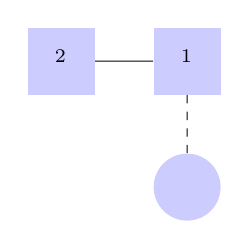
\begin{tikzpicture}
      [scale=.8,auto=left,every node/.style={circle,fill=blue!20}]
      \node[rectangle,minimum size=0.85cm] (n1) at (3,3) {$\tehole^{1}$};
      \node[rectangle,minimum size=0.85cm] (n2) at (1,3)  {$\tehole^{2}$};
      \node[minimum size=0.85cm] (i) at (3,1)  {$\tnum$};
    
      \foreach \from/\to in {n1/n2}
        \draw (\from) -- (\to);
       \foreach \from/\to in {n1/i}
        \draw[dashed] (\from) -- (\to);
    
    \end{tikzpicture}
  \caption{Graph of $C_{ex2} = \{ \tehole^{1} \approx \tnum, ~ \tehole^{1} \approx~ \tehole^{2}\}$}
  \label{fig:reachable-tag}
\end{subfigure}
\begin{subfigure}{.49\textwidth}
  \centering
  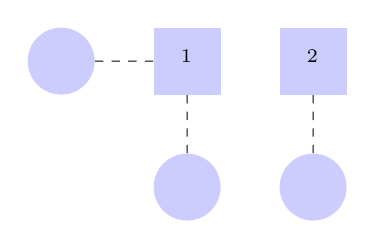
\begin{tikzpicture}
  [scale=.8,auto=left,every node/.style={circle,fill=blue!20}]
  \node[rectangle,minimum size=0.85cm] (n1) at (2,3) {$\tehole^{1}$};
  \node[rectangle,minimum size=0.85cm] (n2) at (4,3)  {$\tehole^{2}$};
  \node[minimum size=0.85cm] (i1) at (4,1)  {$\tnum$};
  \node[minimum size=0.85cm] (i2) at (2,1)  {$\tnum$};
  \node[minimum size=0.85cm] (i3) at (0,3)  {$\tbool$};

   \foreach \from/\to in {n1/i3, n1/i2, n2/i1}
    \draw[dashed] (\from) -- (\to);

\end{tikzpicture}
  \caption{Graph of $C_{ex3} = \{ \tehole^1 \approx \tnum, ~ \tehole^1 \approx \tbool, ~ \tnum \approx~ \tehole^2\}$}
  \label{fig:disjoint-nodes}
\end{subfigure}
\caption{Sample constraint graphs of ground types}
\label{fig:ex2ex3graphs}
\end{figure}

% Constructing a graph of type nodes and adding edges between them has an important caveat: Only $\tehole^{p}$ or types containing at least one $\tehole^{p}$ are added to the graph as nodes. See Figure \ref{fig:ex1ex2graphs} for an illustration. In part (a) of Figure \ref{fig:ex1ex2graphs}, $\tehole^{1}$ and $\tehole^{2}$ are nodes in the graph \textit{linked} by a solid edge, and $\tnum$ is not. Instead, $\tnum$ is more like a \textit{tag} adding additional type information to $\tehole^{1}$. Hence, we use a dotted edge in the illustration to represent this distinction. Since $\tnum$ is constrained to $\tehole^{1}$, the solver can infer using union-find that $\tehole^{2}$ must also contain $\tnum$ in its \textit{PotentialTypeSet}, because $\tehole^{1}$ and $\tehole^{2}$ are part of the same connected component. By contrast, in part (b), $\tehole^{1}$ and $\tehole^{2}$ are both \textit{tagged} with $\tnum$, but because they are not part of the same connected component, the solver will not infer that they share the same \textit{PotentialTypeSet}. Consequently, the solver will correctly not infer that $\tehole^2$ contains $\tbool$ in its \textit{PotentialTypeSet}.

Upon encountering a constraint between two arrow types, we can generate two new constraints on-the-fly: one between the left children of the arrows, and one between the right children of the arrows. For example, given the constraint set $C_{ex4} = \{ \tarr{\tehole^1}{\tehole^2} \approx \tarr{\tehole^3}{\tnum} \}$, we generate the constraints $\tehole^1 \approx \tehole^3$ and $\tehole^2 \approx \tnum$. These constraints can then be used to render the graph depicted in Figure \ref{fig:arrowgraph}. Here, we represent incomplete $Arrow$s as nodes whose types are dependent on their left and right hand sides, which may also be nodes. As an example, we see in Figure \ref{fig:arrowgraph} that $\tarr{\tehole^1}{\tehole^2}$ is represented by a large arrow node containing the node $\tehole^1$ on the left and $\tehole^2$ on the right. 
% Any node linked to an $Arrow$ node can only access its left and right hand sides once they are paired together and wrapped in a binary $\rightarrow$ type. 

With these rules in hand, we can construct graphs for more complex constraint sets. Let us explore the graph of the constraint set $C_{ex1}$ generated from the synthesis of $\ECMV_{ex}$ in section 4.4.8:
$$C_{ex1} = \{ \TUnknown^{exp(2)} \approx \tbool, \TUnknown^1 \approx \tarr{\TUnknown^{\rightarrow_L(1)}}{\TUnknown^{\rightarrow_R(1)}},  \TUnknown^{\rightarrow_L(1)} \approx \tnum, \TUnknown^{exp(0)} \approx \TUnknown^{1}, \TUnknown^{\rightarrow_R(1)} \approx \TUnknown^{exp(3)} \}$$
We provide an illustration of this constraint graph in Figure \ref{fig:C-ex-graph-traversal}. The red edges in Figure \ref{fig:C-ex-graph-traversal} represent all paths that may be followed beginning at $?^1$. 

Suppose we wanted to generate a suggestion for $?^1$ using this graph. This could be achieved by simply traversing all red edges in Figure \ref{fig:C-ex-graph-traversal} to discover potential types. Note that potential types discovered within the left and right hand side of the $Arrow$ node must be wrapped pairwise in an $\rightarrow$ type before being added to $?^1$'s list of potential types. Following these edges generates the following set of potential types for $?^1$: $\{  ?^0, ?^1, \tarr{\tnum}{?^3}, \tarr{\tehole^{\rightarrow_{L(1)}}}{?^3}, \tarr{\tnum}{\tehole^{\rightarrow_{R(1)}}}, \tarr{\tehole^{\rightarrow_{L(1)}}}{\tehole^{\rightarrow_{R(1)}}}  \}$. Notice that after exploring the arrow, our number of potential types have grown rapidly!

\begin{figure}[htb!]
\centering
\captionsetup[subfigure]{justification=centering}
\begin{subfigure}{.49\textwidth}
        \centering
      \begin{tikzpicture}[remember picture,
  inner/.style={rectangle,draw=blue!50,fill=blue!20,thick,inner sep=3pt,minimum size=0.85cm},
  innercirc/.style={circle,draw=blue!50,fill=blue!20,thick,inner sep=3pt,minimum size=0.85cm},
  outer/.style={draw=green,fill=green!20,thick,inner sep=10pt}
  ]
  \node[outer,draw=green] (A) {
    \shortstack{
        $Arrow$\\
        \begin{tikzpicture}
          \node [inner] (n1)  {$\tehole^{1}$};
          \node [inner,right=of n1] (n2) {$\tehole^{2}$};
          % \draw[red,thick,->] (n1) -- (n2);
        \end{tikzpicture}
    }
  };
  \node[outer,draw=green,below=of A] (B) {
    \shortstack{
        $Arrow$\\
        \begin{tikzpicture}
          \node [inner] (n3)  {$\tehole^{3}$};
          \node [innercirc,right=of n3] (i) {$\tnum$};
          % \draw[red,thick,->] (n3) -- (i);
        \end{tikzpicture}
    }
  };
  \draw (n1) -- (n3);
  \draw[dashed] (n2) -- (i);
   \draw[thick] (A) -- (B);
\end{tikzpicture}
\caption{Expanded constraint graph of\\ $C_{ex3} = \{ \tarr{\tehole^1}{\tehole^2} \approx \tarr{\tehole^3}{\tnum} \}$}
\label{fig:arrowgraph}
\end{subfigure}
\begin{subfigure}{.49\textwidth}
  \centering
  \begin{tikzpicture}[remember picture,
  tag/.style={circle,draw=blue!50,fill=blue!20,thick,inner sep=3pt,minimum size=0.85cm},
  holey/.style={rectangle,draw=blue!50,fill=blue!20,thick,inner sep=5pt,minimum size=0.85cm},
  outer/.style={draw=green,fill=green!20,thick,inner sep=10pt},
  ]
  \node[holey] (hole1) {$\tehole^1$};
  \node[holey, right=of hole1] (hole0) {$\tehole^0$};
  \node[outer, below=of hole1] (Arrow) {
    \shortstack{
        $Arrow$\\
        \begin{tikzpicture}
          \node [holey] (holeL1)  {$\tehole^{\rightarrow_{L(1)}}$};
          \node [holey, right=of holeL1] (holeR1) {$\tehole^{\rightarrow_{R(1)}}$};
        \end{tikzpicture}
    }
  };
 \node[tag, below=of holeL1] (num) {$\tnum$};
 \node[holey, below=of holeR1] (hole3) {$\tehole^3$};
 \node[holey, right=of holeR1] (hole2) {$\tehole^2$};
 \node[tag, below=of hole2] (bool) {$\tbool$};
  \draw[draw=red] (hole1) -- (hole0);
  \draw[draw=red] (hole1) -- (Arrow);
  \draw[dashed, draw=red] (num) -- (holeL1);
  \draw[draw=red] (hole3) -- (holeR1);
  \draw[dashed] (bool) -- (hole2);
\end{tikzpicture}
% \caption{Constraint graph of\\ 
% $C_{ex1} = \{ \TUnknown^{exp(2)} \approx \tbool, \TUnknown^{exp(0)} \approx \TUnknown^{1},$ \\
% $\TUnknown^1 \approx \tarr{\TUnknown^{\rightarrow_L(1)}}{\TUnknown^{\rightarrow_R(1)}},  \TUnknown^{\rightarrow_L(1)} \approx \tnum,$ \\
% $\TUnknown^{\rightarrow_R(1)} \approx \TUnknown^{exp(3)} \}$}
\caption{Constraint graph of $C_{ex1}$}
\label{fig:C-ex-graph-traversal}
\end{subfigure}
\caption{Sample constraint graphs including binary types}
\label{fig:ex1ex2graphs}
\end{figure}

\subsubsection{PotentialTypeSets and the Graph Construction Algorithm}
Now that we have a clear approach to generating constraint graphs, how might we represent the types that are adjacent to each node? One approach would be to simply store an adjacency list or matrix. However, we'd like to be able to efficiently store all potential hole fillings that can be derived from a type hole's connected components. Recall the rapid growth of potential types discovered for $?^1$ from the graph of $C_{ex1}$ in Figure \ref{fig:C-ex-graph-traversal}. Since the set of potential types can grow at a combinatorial rate, we define a new, condensed data structure to house our potential type hole fillings without loss of information: a \emph{PotentialTypeSet}.

A \textit{PotentialTypeSet} is a recursive data structure representing the potential solutions for a type hole, inferred from type constraints. A single \emph{PotentialTypeSet} contains \emph{all} of the potential fillings for its associated type hole. To facilitate this, rather than ever substituting types during unification, which results in a loss of information, we continuously extend some \emph{PotentialTypeSet}. We provide a formalization of \textit{PotentialTypeSet}, \textit{PotentialType}, and their extension below in Figure \ref{fig:possible_type_sets}.

\begin{figure}[hbt!]
\centering
\vspace{-3px} 
$\arraycolsep=4pt\begin{array}{lll}
PotentialTypeSet~~ s & ::= 
single(t) ~\vert~ 
cons(t, s)
\\
PotentialType~~ t & ::= 
  \tnum ~\vert~
  \tbool ~\vert~
  \tehole^p ~\vert~
  \tarr{s}{s}
  \\
\end{array}$
\label{fig:syntax_possible_type_sets}
\vspace{5px}
\hrule
\[\begin{array}{rcl}
    single(\tarr{s_1}{s_2}) ~\amalg~ single(\tarr{s_3}{s_4}) & = & single({\tarr{(s1 ~\amalg~ s3)}{(s2 ~\amalg~ s4)}}) \\
    single(t) ~\amalg~ single(t') & = & cons(t, single(t')) \\
    cons(t,s) ~\amalg~ single(t) & = & cons(t, s) \\
    cons(\tarr{s_1}{s_2}, s) ~\amalg~ single(\tarr{s_3}{s_4}) & = & cons(\tarr{(s1 ~\amalg~ s3)}{(s2 ~\amalg~ s4)} , s) \\
    cons(t,s) ~\amalg~ cons(t',s') & = & cons(t,s) ~\amalg~ single(t') ~\amalg~ s' \\
\end{array}\] 
\caption{Syntax of PotentialTypeSets, PotentialTypes, and their Merging}
\vspace{5px} 
\label{fig:possible_type_sets}
\vspace{-5px}
\end{figure}

With this in hand, we formalize the intuitions discussed in section 4.5.1 in a graph construction algorithm. This algorithm accumulates a mapping from incomplete types, which represent our nodes, to their \emph{PotentialTypeSet}, which represents a subset of nodes reachable from a given incomplete type. Whenever we attempt to create a traversable edge or a solution edge between nodes, we retrieve the \emph{PotentialTypeSet}s of all involved nodes, compute the result of merging them, and update our graph accordingly. We assume the existence of a \lstinline{Map.add} function that adds a new element to the supplied map if it does not already exist, and otherwise does not change any values. The corresponding definition is provided in Figure \ref{fig:algcode_construct_graph}

\begin{figure}[hbt!]
\begin{lstlisting}[escapeinside={(*}{*)}]
let rec construct_graph (~graph=Map.empty(), constraints) =
    match constraints with
    | [] -> graph
    | hd::tl -> (
        (match hd with
        | ((*$\tarr{t1_L}{t1_R}$*), (*$\tarr{t2_L}{t2_R}$*)) ->
            construct_graph(~graph, (((*$t1_L$*), (*$t2_L$*)))::(((*$t1_R$*), (*$t2_R$*)))::tl)
        | ((*$\tehole^{p}$*) as hole, t)
        | (t, (*$\tehole^{p}$*) as hole) ->
            let graph = Map.add(graph, hole, hole) in
            if (contains_hole(t)) then (
                let graph = Map.add(graph, t, t) in
                let graph = create_traversable_edge(graph, t, hole) in
                construct_graph(~graph, tl)
            ) else (
                let graph = create_solution_edge(graph, hole, t) in
                construct_graph(~graph, tl)
            )
        | _ -> construct_graph(~graph, tl))

\end{lstlisting}
\hrule
\caption{Constraint graph creation algorithm of type hole inference}
\label{fig:algcode_construct_graph}
\end{figure}

\subsubsection{Computing PotentialTypeSets Using Constraint Graphs} 
The function \lstinline{construct_graph} builds a mapping from each type hole to a \emph{PotentialTypeSet} containing a subset of its connected component. However, in order to generate all potential type hole fillings, we require that each \emph{PotentialTypeSet} represent the entire connected component. One method to expand our \emph{PotentialTypeSet}s would be to conduct a depth first search of our graph. Instead of this, we choose to simply augment our current approach using union find, yielding a version of \lstinline{construct_graph} that is reminiscent of Huet's unification algorithm \cite{Huet}.

In order to change our graph construction algorithm to a constraint solver, all we need to do is update our definitions of \lstinline{create_traversable_edge} and \lstinline{create_solution_edge} to use represent each potential type set using union find. In order to accommodate this change, minor adjustments must be made to the definitions presented in Figure \ref{fig:possible_type_sets} to create union findable possible type sets and their extension logic, $\amalg_{UF}$. These definitions are left to the supplemental material for reference.

An additional step is taken to mark type holes with an error if their \emph{PotentialTypeSet} contains a cycle that is not a self loop. In Hindley-Milner type inference this is referred to as the occurs-check.

After our union find based \lstinline{construct_graph} and occurs check marking have been completed, we are ready to identify the solvability of our type holes. We consider type holes solvable if their \textit{PotentialTypeSet} contains at most one type that is not a hole. On the other hand, if a type hole's \textit{PotentialTypeSet} contains multiple conflicting types, or if the type hole fails the occurs check, then it is considered unsolvable. In both cases,  feedback can be provided as in Figure \ref{fig:editor_conflict}.

% \subsubsection{Other Binary Types}
% Suppose we wanted to extend our definitions of constraint generation and solving to contain binary products as discussed in section 2.2. This would require an extension of our constraint generation rules and definitions of \emph{PotentialTypeSet}s. We follow the same procedures in section 4.4 and introduce a new matched product judgement that constrains inputted holes to their matched product form. In order to extend \emph{PotentialTypeSet}s to support binary products, we must slightly adjust our definitions to be more general across different binary type operators. The resulting rules are very similar to those discussed earlier, and are also consequently left for review in the supplemental material.

\subsection{Polymorphic Generalization}
% In order to extend our definitions of \emph{PotentialTypeSet}s to allow parametric polymorphism, we simply include a new ground type: $\TVar$.
% \begin{center}
% $\arraycolsep=4pt\begin{array}{lll}
% PotentialType~~ t & ::= 
%   \dots \mid \TVar
% \end{array}$
% \end{center}
% By representing all type variables this way, we enforce that type variables are only consistent with type holes and each other. 
For the sake of minimality, our discussion above did not formalize parametric polymorphism. Integration of parametric polymorphism into type inference is well-understood. Type hole inference 
creates only one particularly interesting wrinkle, having to do with the common practice of implicitly generalizing unconstrained type inference variables, here type holes. With the inclusion of expression holes in our system, we need to be a bit more careful in when we generalize. Consider the following expression:
$$\ECLam{x}{\TUnknown^1}{\EEHole^2}$$
We can see that $\TUnknown^1$ is not constrained. Suppose that we were to suggest the implicitly universally quantified type variable $'a$ as a type hole filling for $?^1$. It is unlikely that the user accepts this suggestion because it is unlikely that the user intends to write the identity function!
The fact there are not yet any constraints does not imply that there will not be once the expression hole is filled.

To address this, we need to reason as if there are any number of \emph{unknown constraints} coming from expression holes.  This status can be represented with a new type of constraint: the $\mathtt{etc}$ constraint, which we add to our syntax of \emph{PotentialTypes} below. 
\begin{center}
$\arraycolsep=4pt\begin{array}{lll}
PotentialType~~ t & ::= 
  \dots \mid \mathtt{etc}
\end{array}$
\end{center}
When an expression hole appears, all type holes in the typing context are constrained to $\mathtt{etc}$. If a type hole $?^p$ is constrained to $\mathtt{etc}$, it cannot be generalized to a type variable.

% \subsubsection{User Interaction and Conflict Highlighting}
% To further the goal of helping users repair their programs, it would be beneficial to assign blame by highlighting the portions of the program responsible for the unsolved status of a \textit{PotentialTypeSet}. To allow this, constraints could be extended to contain the unique identifier of the expression from which they originated. Highlighting all expressions of the program which resulted in an unsolved \textit{PotentialTypeSet}, rather than attempting to localize the error to one particular expression, would result in less confusion and give the user more clues to discover the true source of a type error.
%These identifiers effectively act as reasons for edges within our constraint graph, enabling us to describe the exact series of reasons that caused the inference algorithm to conclude a type hole's solution status.



